\section{Software}
\label{sec:chapterexample}

\subsection{Übersicht}
Das System besteht aus mehrere Hardware- und Softwarekomponenten die zusammenarbeiten müssen (\seeref{fig:echosystem}). Die Kommunikation zwischen den Knoten ist von TLS immer gewährleistet. Die einzelne Komponente werden in den nächsten Kapiteln genauer beschrieben.

\begin{figure}[htb!]
	\begin{center}
		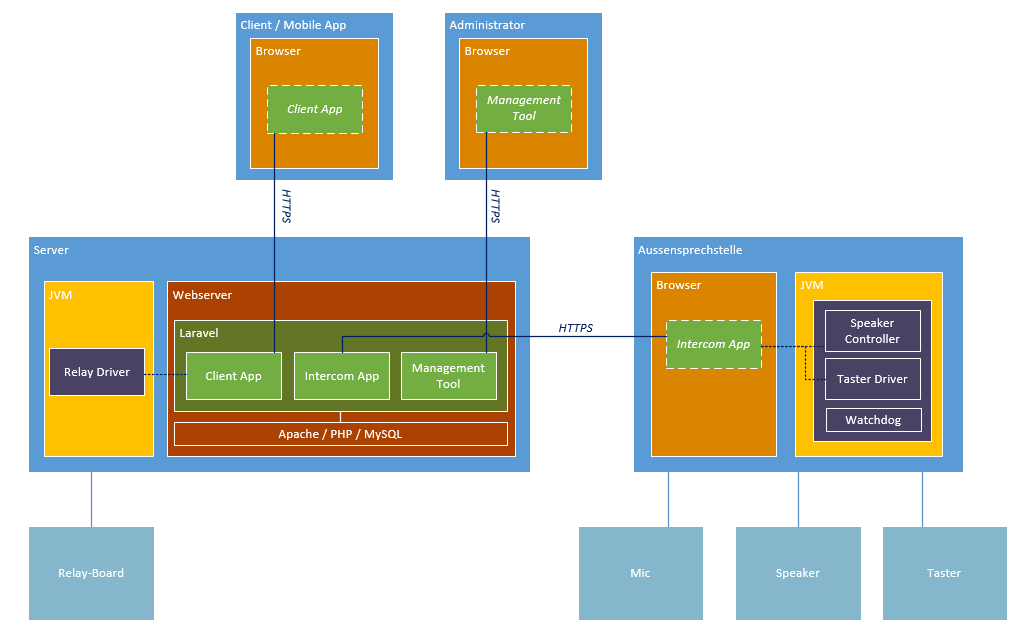
\includegraphics[width=1\textwidth]{ecosystem}
		\caption[Software / Hardware Ecosystem]{Software / Hardware Ecosystem}
		\label{fig:echosystem}
	\end{center}
\end{figure}

\subsection{Programmiersprachen}
Das System besteht aus mehrere Programme und Dienste. Für die Entwicklung werden folgende Programmiersprachen eingesetzt:
\begin{itemize}
	\item Java
	\item Javascript
	\item PHP
\end{itemize}
Im Verbindung mit PHP kommt natürlich die Markup-Languages HTML5/CSS, welche für die graphische Darstellung der Webapplikationen notwendig ist.

\subsubsection{Java}
Alle Dienste die Serverseitig und ohne Interaktion mit dem Enduser ausgeführt werden, werden in Java programmiert. Als stark typisierte und Objektorientierte Programmiersprache eignet sich Java für dieses Projekt. Für Java sind auch unzählige Libraries verfügbar, insbesondere für die Hardware Steuerung der Raspberry Pi. Eine zweite Variante wäre Python gewesen, die auch das Raspberry sehr gut unterstüzt. Python ist aber zu wenig typisiert und für eher kleinere Softwarestücke gedacht.

\subsubsection{PHP/Javascript}
Die Enduser Applikation sowohl auch die Applikation bei der Aussensprechstelle werden Web-Applikationen sein. Dies ermöglicht eine schnelle und zeitgemässe Softwareentwicklung. Für dieses Projekt ist die System-Eingriffstiefe von Webapplikationen jedenfalls ausreichend. Es muss lediglich Zugriff auf Mikrofon, Lautsprecher und Kamera garantiert werden. Ein weiteres Punkt zugunsten einer Webapplikation ist die Cross-Plattform Kompatibilität. 
\\
Aus diesem Grund haben wir uns für PHP (Objektorientiert) im Kombination mit Javascript/HTML/CSS Entschieden. Eine zweite Variante wäre Java EE gewesen. Java EE eignet sich aber vor allem für grosse Softwarelösungen und bietet als gesamten Framework vieles mehr als was dieses Projekt benötigt. 
\\
\subsubsection{PHP Framework: Laravel}
Für die Entwicklung der Webapplikationen wird Laravel als PHP Framework eingesetzt. Laravel ist ein Open-Source PHP Web-Application-Framework, die sich für kleine bis zu mittelgrosse Projekte eignet. Laravel beruht auf dem Modell-View-Controller-Muster und ermöglicht eine Objektorientierte Programmierung in PHP.

\subsection{Skripts}


\subsection{Webapplikationen}

\subsubsection{Client Webapplikation}
Der Bewohner muss über eine Applikation verfügen, die auf dem Tablet oder Handy ausführbar sein muss. Mithilfe dieser App muss der Enduser im Stande sein, sich mit alle Aussensprechstellen sich verbinden zu können, das Video Signal von der Kamera erhalten, die Türe öffnen und mit der Person bei der Türe kommunizieren können.
\\
\begin{figure}[htb!]
	\begin{center}
		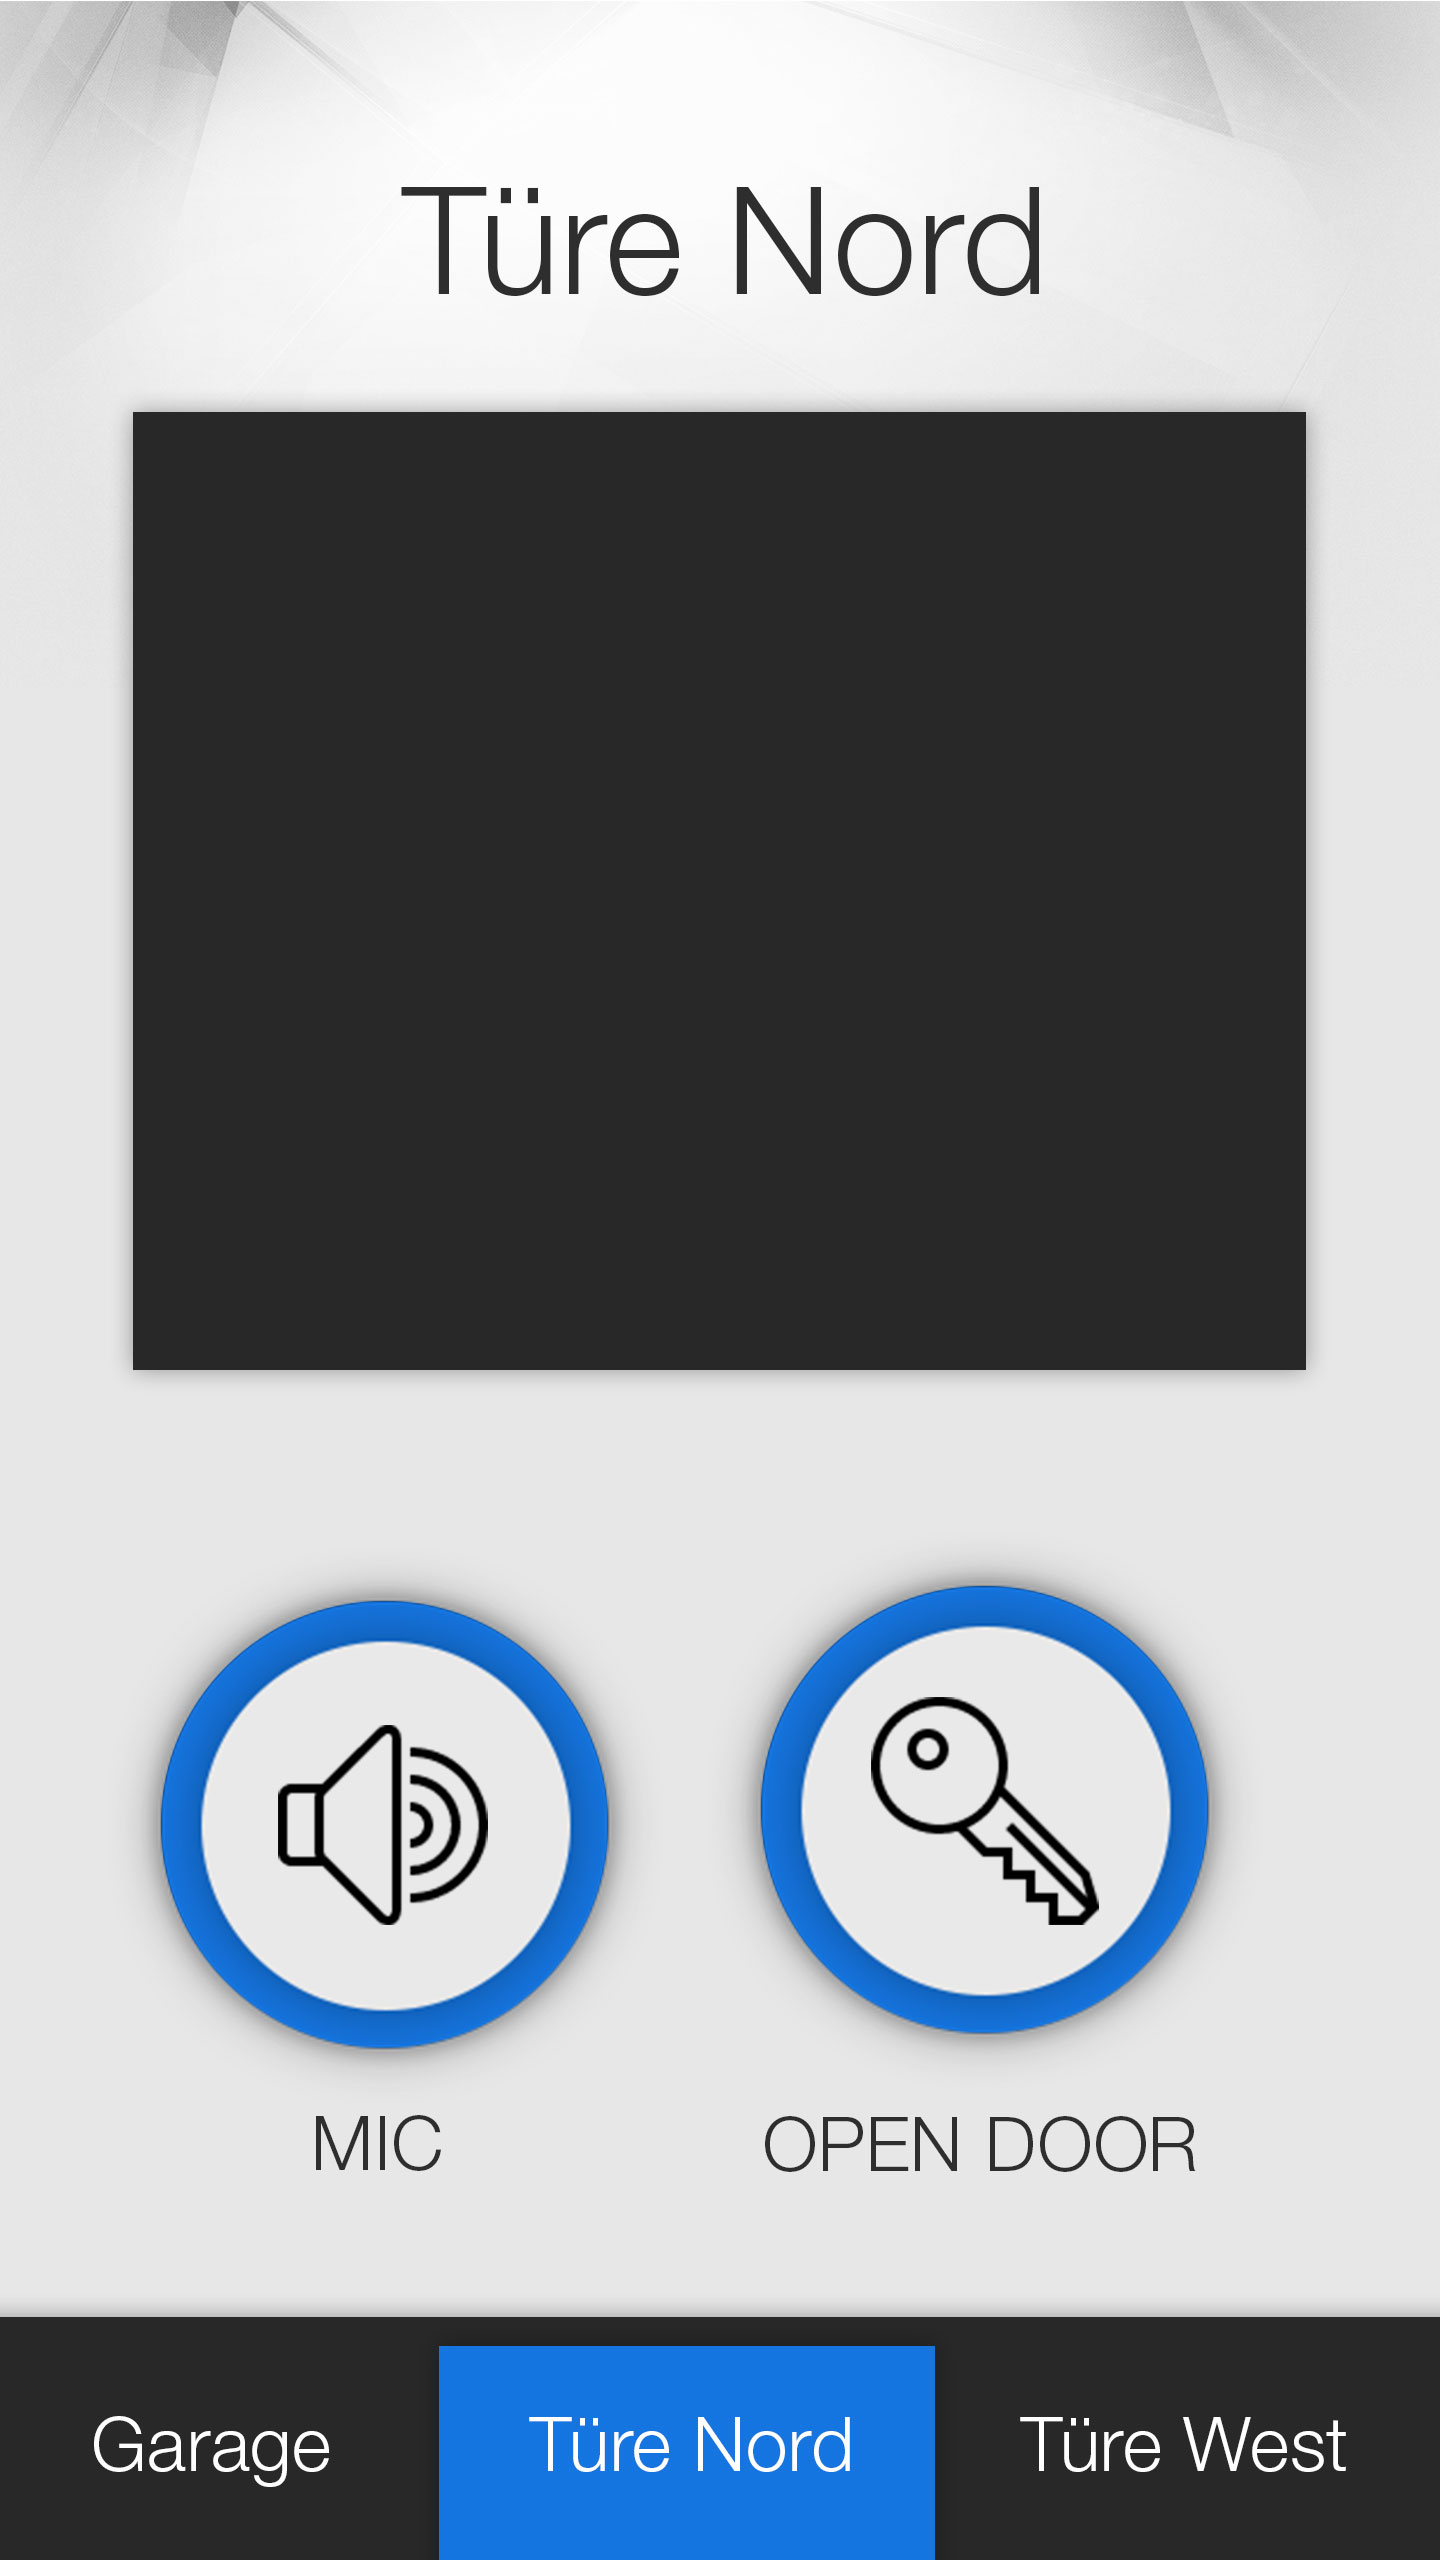
\includegraphics[width=0.3\textwidth]{clientDemo}
		\caption[Erste Designentwurf der Client App]{Erste Designentwurf der Client App}
		\label{fig:clientDemo}
	\end{center}
\end{figure}



\newpage